\documentclass[10pt, a4paper]{article}

% --- Typography: Times New Roman ---
\usepackage[utf8]{inputenc}
\usepackage[T1]{fontenc}
\usepackage{mathptmx} 

% --- Layout ---
\usepackage[margin=2.5cm]{geometry}
\usepackage{amsmath, amssymb}
\usepackage{graphicx}
\usepackage{booktabs}
\usepackage{siunitx}
\usepackage{enumitem}
\usepackage{titlesec}

% --- Centering Style ---
\titleformat{\section}{\large\bfseries\centering}{}{0em}{}
\titleformat{\subsection}{\bfseries\centering}{}{0em}{}
\setlist[itemize]{noitemsep, leftmargin=1.5em}

\begin{document}

\begin{center}
    {\small PhysEng Lab | SQUID Experiment} \\
    {\small \textbf{Gregorio Jaca and Peter Tallosy}} \\
    {\small \textit{\today}}
    
    \vspace{2em}
    
    {\Large \textbf{LAB NOTES: SQUID CHARACTERISATION}}
\end{center}

\vspace{1.5em}

\section*{1. Junction V-I Characteristics}
We initiated the measurement in the superconducting (SC) regime, observing the transition as the temperature increased towards the non-SC state. 
\begin{itemize}
    \item \textbf{Setup:} Drive current set to \SI{120}{\micro\ampere} with a \SI{10}{\kilo\ohm} bias resistor.
    \item \textbf{Energy gap:} The SC regime is governed by the energy gap $\Delta(T) \propto T_c \sqrt{1 - T/T_c}$, which represents the binding energy of Cooper pairs. The modulation of the critical current allows for the mapping of the density of states (DOS) threshold.
    \item \textbf{Params:} From the I-V curves (Fig. 1), the critical current was determined to be $I_c = \SI{82}{\micro\ampere}$.
\end{itemize}

\begin{center}
    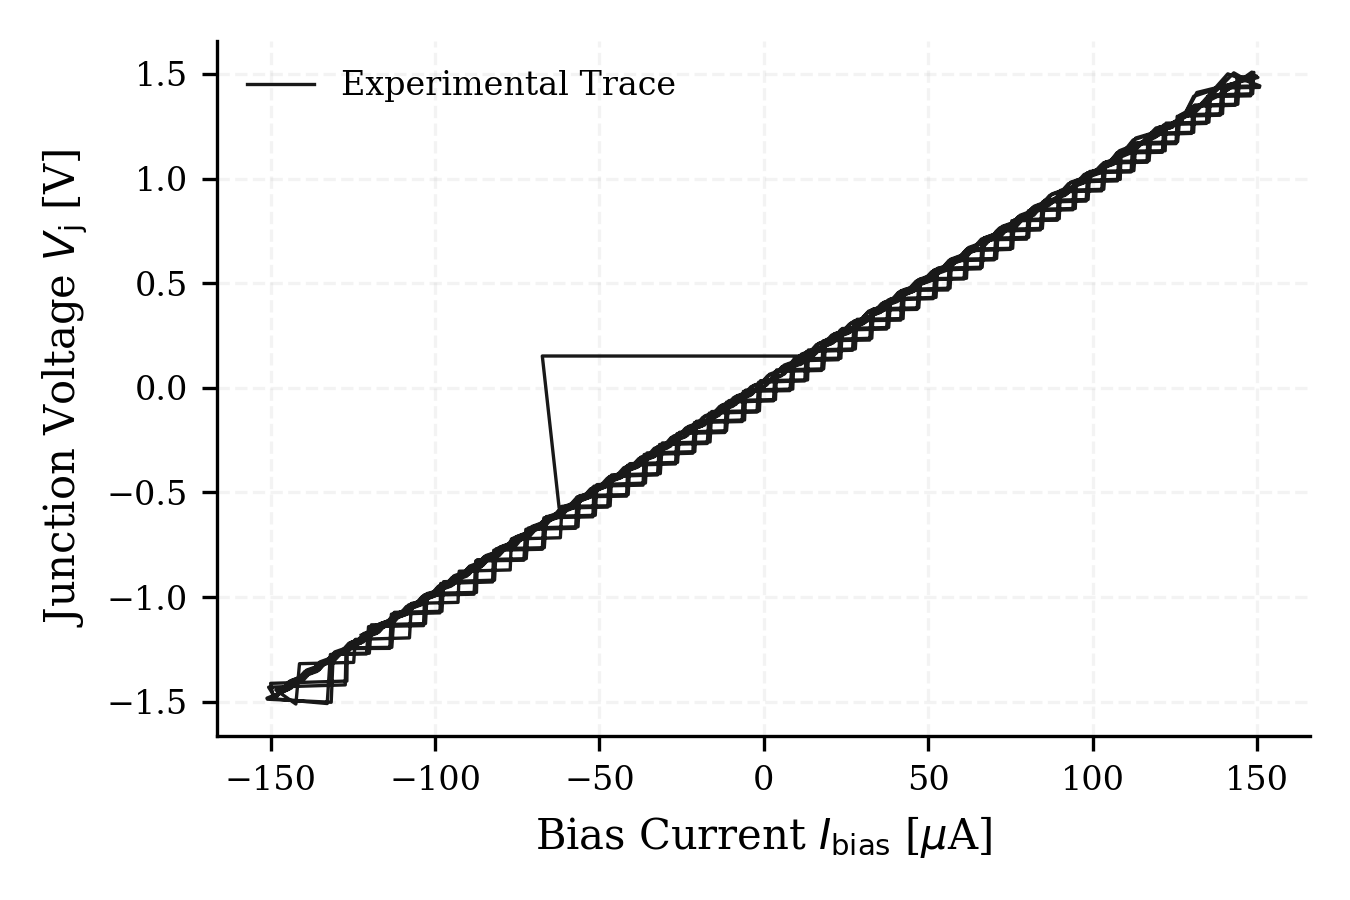
\includegraphics[width=0.55\textwidth]{task1_iv.png} \\
    \footnotesize \textit{Fig 1: Single Josephson Junction I-V trace showing SC transition.}
\end{center}

\section*{2. SQUID I-V Response}
The flux bias current $I_b$ was swept $\pm\SI{300}{\micro\ampere}$ to tune the critical current of the SQUID loop. Adaptive gain was manually applied at the oscilloscope to maintain signal resolution across the modulation depth.

\begin{center}
    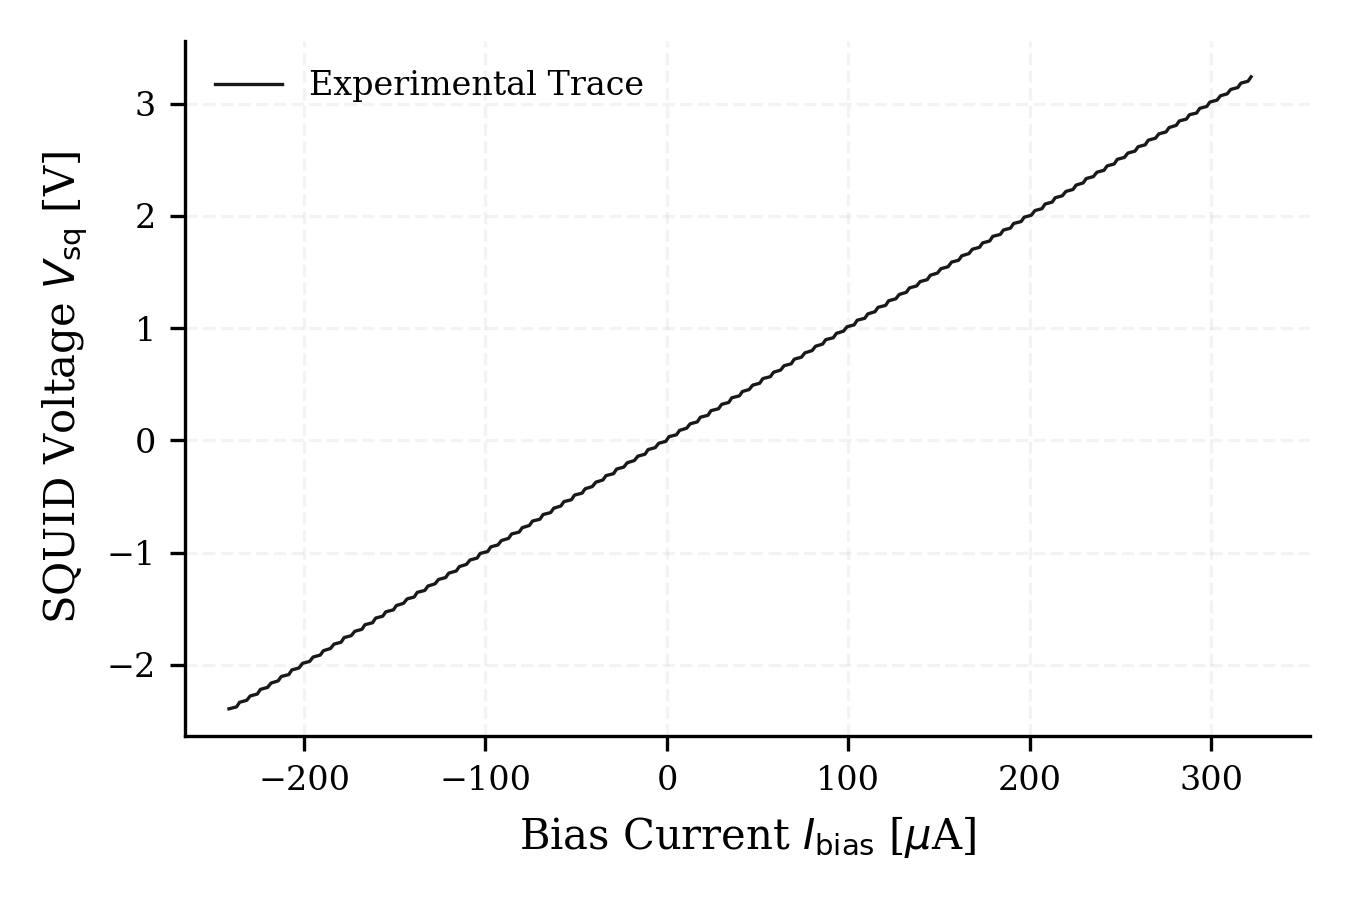
\includegraphics[width=0.55\textwidth]{task2_iv.png} \\
    \footnotesize \textit{Fig 2: SQUID I-V characteristics under varying magnetic flux.}
\end{center}

\section*{3. Flux response and Mutual Inductance}
A \SI{41}{Hz} triangle drive was used for flux biasing, resulting in an interference response of approximately \SI{400 \pm 100}{Hz}, indicating the traversal of multiple flux quanta within a single sweep.

\begin{center}
    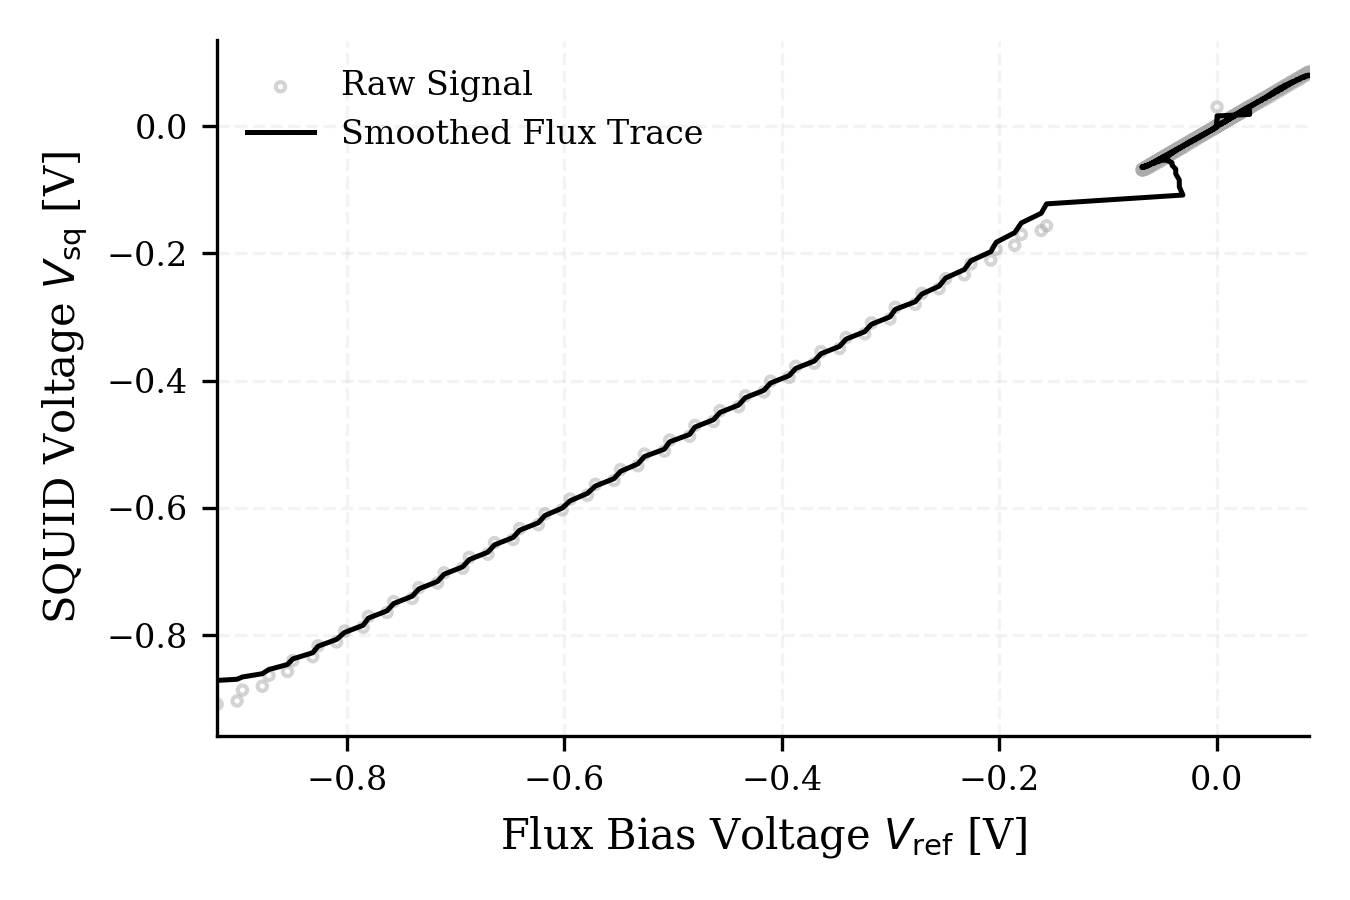
\includegraphics[width=0.55\textwidth]{task3_flux.png} \\
    \footnotesize \textit{Fig 3: Intereference pattern as a function of flux bias voltage $V_{\mathrm{ref}}$.}
\end{center}

\subsection*{Inductance Extraction (Task 3)}
Automated peak detection on 14 analyzed periods yielded the following results:
\begin{center}
\begin{tabular}{ll}
    \toprule
    \textbf{Metric} & \textbf{Value} \\
    \midrule
    Bias Voltage Period $\Delta V_{\mathrm{ref}}$ & \SI{0.8293}{V} \\
    Bias Current Period $\Delta I_{\mathrm{flux}}$ & \SI{82.93}{\micro\ampere} \\
    \textbf{Mutual inductance $M$} & \textbf{\SI{24.94}{nH}} \\
    \bottomrule
\end{tabular}
\end{center}

\vspace{1em}
The extracted $M$ is highly consistent with manual Gregorian-style estimation based on $\Delta I_{\mathrm{flux}} = \Phi_0/M$.

\end{document}
